\chapter{Generative and Performative Algorithms}

Two main paradigms of algorithmic architectural design are clearly dominant; generative design and performative design \cite{fasoulaki08}. Generative design is the essential \emph{rule-based\footnote{Consisting of a solid set of consecutive instructions that govern an action to produce a desired outcome}} algorithmic form of algorithmic architecture. It is governed by repetitive patterns, equations and shape transformations.  Performative design on the other hand, is optimisational; modifying and reshaping to adapt to a certain simulated environment, or to achieve a specific level of performance for specfific building functions.

\section{Generative Algorithm}

Generative architecture can be defined as a design process involving generative systems in the form of a computer program that can be fully automated or step-by-step controlled. It would have an algorithm (rule) governing the transformations of initial shapes through variables or parameters; `generating' results, and selecting the best variant according to the given criteria. \cite{arida04}

Generative algorithms are visual in nature; they are systems which define, manipulate and --- most imprtantly --- react to and are driven by shapes and geometries. This is in contrast with performative algorithms, which are driven by building performance, which is of a more numerical nature. 

The key components of generative design are the systems which define the method of form exploration. They can be defined as scripts or sets of geometrical transformations \cite{arida04}. These systems --- as mentioned earlier --- are rule based, essentially formal or visual, and are often emulations of natural processes or systems; such as biologcal evolution and mathematical patterns. Some of the more popular systems --- as far as architectural design is concerned --- widely used today include Cellular Automata, L-Systems, Voronoi Diagrams, Fractals and Shape Grammars.

\clearpage
\subsection{Cellular Automata}

``Cellular Automata is a computational method which can simulate the process of growth by describing a complex system by simple individuals following simple rules. The concept of simulating growth was introduced by John von Neumann (1951) and further developed by Ulam (1962) in the are of simulating multi-state machines. The concept gained great popularity when Martin Gardner (1970) John Conway's ``Life'', a game that generated two dimensional patterns''\cite{krawczyk02}. Later on, Stephen Wolfram would begin research on the subject in 1984, to write a book on the subject called \emph{A New Kind of Science} \cite{wolfram02}. The book would discuss the patterns created by cellular automata as simple rules capable of generating extremely complex patterns that mimic patterns of growth occurring in nature, among other things; describing his findings as a new paradigm of scientific research touching on numerous fields of science.

\begin{figure}[htbp]
\centering
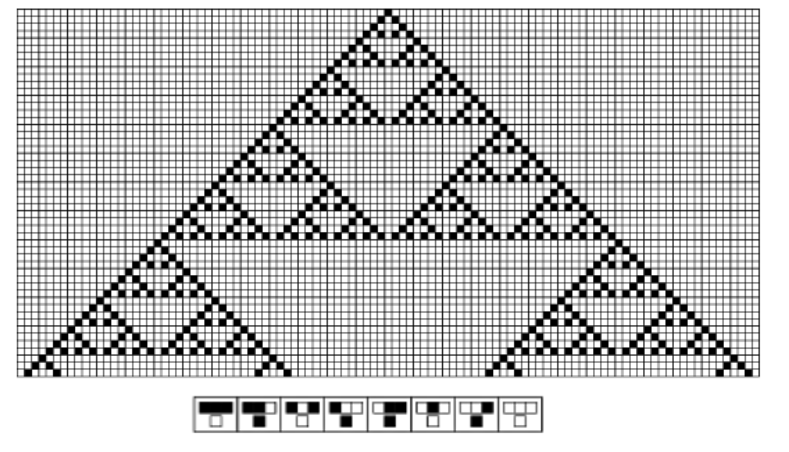
\includegraphics[width=\textwidth]{./Images/1-CellAutoEg}
\caption[Cellular Automaton]{An example of cellular automata showing (a) the sequence of generations and (b) the governing rule.\cite{wolfram02}}
\label{CAEg}
\end{figure}

The concept of cellular automata is that an initial configuration of at least one cell occupying an empty space would evolve and procreate into a pattern using a rule that decides birth, life and death cells through the preceding related cells (Fig. \ref{CAEg}). The pattern shown is a two dimensional growth pattern used by Stephen Wolfram. Other forms of cellular automata generation include 3-dimensional ones, which are the architects main interest.

The method of generation in 3-dimensional cellular automata remains basically the same as with 2-dimensional ones; with an initial configuration of blocks occupying spaces and a rule that governs the shape of each generation (Fig \ref{3dCA}).

\begin{figure}[htbp]
\centering
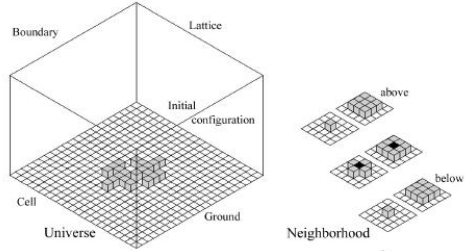
\includegraphics[width=0.7\textwidth]{./Images/2-3dCA}
\caption[3-Dimensional Cellular Automata]{3-Dimensional cellular automata and terminology.\cite{krawczyk02}}
\label{3dCA}
\end{figure}

The utilisation of basic rules of cellular automata however does not suffice to produce architecturally sound models with appropriate internal spaces in most cases (Fig \ref{3dCAArch}). In order to produce such forms, a degree of optimisation and modification is required. A fairly simple but effective solution is manipulation of cell interpretation. Examples of such manipulation are stretching cells to overlap forming adequate internal spaces, merging the overlapping cells and interpreting the envelope of merged cells as splines (Fig \ref{CA Optimisation}).

\begin{figure}[htbp]
\centering
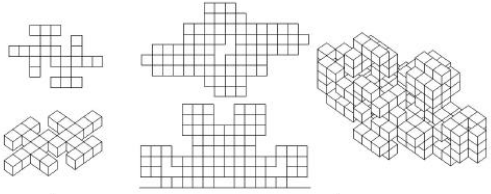
\includegraphics[width=0.7\textwidth]{./Images/3-3dCAArch}
\caption[Cellular Automata Architectural Inadequacy]{An example of CA rules inadequacy for architectural forms without modification \cite{krawczyk02}}
\label{3dCAArch}
\end{figure}


\begin{figure}[htbp]
\centering
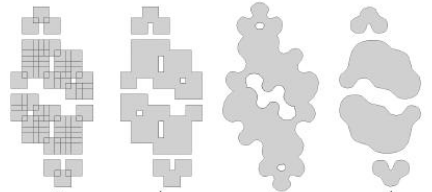
\includegraphics[width=0.7\textwidth]{./Images/4-3dCAArchOpt}
\caption[Cellular Automata Architectural Optimisation]{Optimisation of cell interpretation for architectural form \cite{krawczyk02}}
\label{CA Optimisation}
\end{figure}

Multiple interpretations of the manipulated generations (Fig \ref{CA ArchForm}) were created with structural support. The architectural forms shown appear more developed, nevertheless; it was subject to several modifications of the original cellular automata model which required user intervention at early stages of the process, which would prove CA to be a rather raw method of architectural form generation.

\begin{figure}[htbp]
\centering
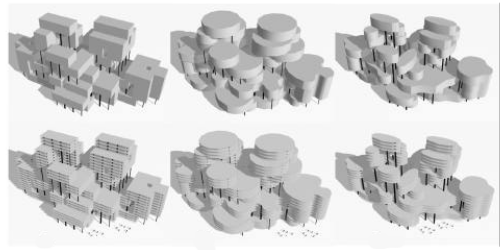
\includegraphics[width=\textwidth]{./Images/5-3dCASpaces}
\caption[Architectural Interpretation of CA Generations]{Architectural Interpretation of CA Generations \cite{krawczyk02}}
\label{CA ArchForm}
\end{figure}

\clearpage
\subsection{Voronoi Diagrams}

``Considered as early as 1644 by Ren\'{e} Descartes but are named after the Russian Mathematician Georgy Fedoseevich Voronoi who studied and defined the general n-dimensional\footnote{\emph{Euclidean Space}: The definition of all points in space by three coordinates; namely $x,y \text{ and } z$} case in 1907''\cite{fasoulaki08}. A Voronoi Diagram is a way of decomposing a space into regions\footnote{Voronoi Diagrams are a class of patterns called Dirichlet tessellations}, this process initiate with a set of points in space; called generating points, the partitioning lines are then drawn from an equal distance from the aforementioned points creating polygons or cells (Fig. \ref{VDiag}).

\begin{figure}[htbp]
\centering
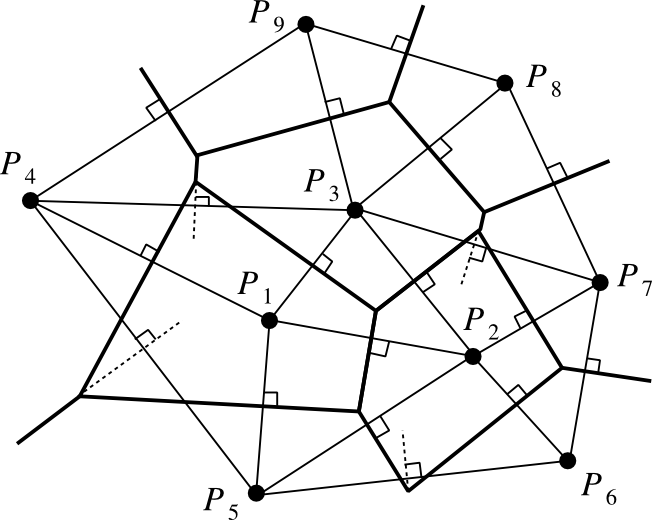
\includegraphics[width=0.8\textwidth]{./Images/6-VoronoiDiagram}
\caption[Voronoi Diagram]{Voronoi Diagram \cite{fujita00}}
\label{VDiag}
\end{figure}

Voronoi Diagrams are naturally occurring patterns such as crystalline formations, bee honeycombs and animal coat patterns among other things, making it a suitable model of form generation and optimisation as well in terms of structure \cite{friedrich08} and environmental performance\label{NaturalOpt}. The main form of utilisation however is that of internal space division or partitioning (Fig. \ref{VDInternal}) and urban design and planning (Fig. \ref{VDUrban})

Although the common form of utilisation of Voronoi Diagram might denote a 2-dimensional constraint, it is also used in 3-dimensional space generating surfaces points in 3D space.

\begin{figure}[htbp]
\centering
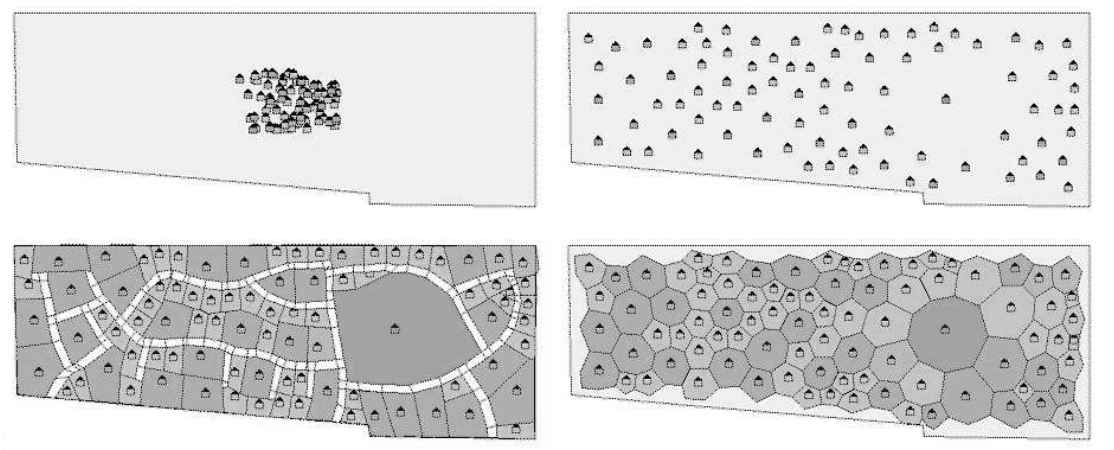
\includegraphics[width=\textwidth]{./Images/7-UrbanVoronoi}
\caption[Voronoi Diagram and Urban Design]{An example of Voronoi Diagram utilisation in urban design (with manual optimisation of final results) \cite{friedrich08}}
\label{VDUrban}
\end{figure}

\begin{figure}[htbp]
\centering
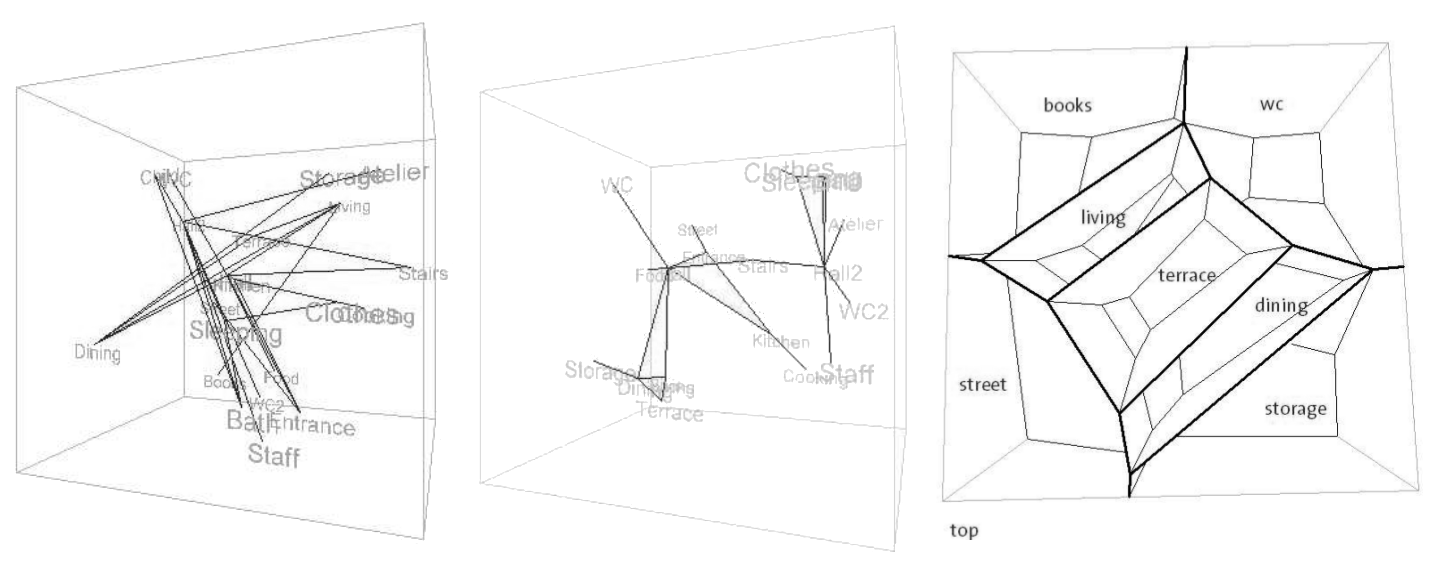
\includegraphics[width=\textwidth]{./Images/8-StructureVoronoi}
\caption[Voronoi Diagram Space Decomposition]{An example of Voronoi Diagram internal space decomposition \cite{friedrich08}}
\label{VDInternal}
\end{figure}

\clearpage
\subsection{Fractals}

``Fractal Geometry is the study of mathematical shapes that display a cascade of never-ending, self-similar, meandering\footnote{\emph{Meander}: to follow a winding or intricate course \cite{merriam03}} detail as one observes them more closely\ldots Fractal geometry is a rare example of technology that can reach into the core of design composition'' \cite{bovill96}.

Originated by Benoit B. Mandelbrot in 1975 \cite{fasoulaki08}, the term \emph{fractals} defines a mathematical rule to produce geometrical shapes that are self-similar\footnote{Reduced copy of the whole}. A fractal is produced by defining an initiator shape and a rule that replaces this shape with a smaller set of copies of the original shape, such as a symmetrical combination of two copies of the original shape. The process goes on in recursion and repetition with virtually no limit to the number of iterations. Examples of this process are: the Koch curve (Fig. \ref{KochCurve}), Sierpinski Gasket, Contor Sets and Julia Sets (Fig. \ref{Fractal} \subref{JuliaSets}).

\begin{figure}[htbp]
\centering
	\subfloat[Fern Fractal]{{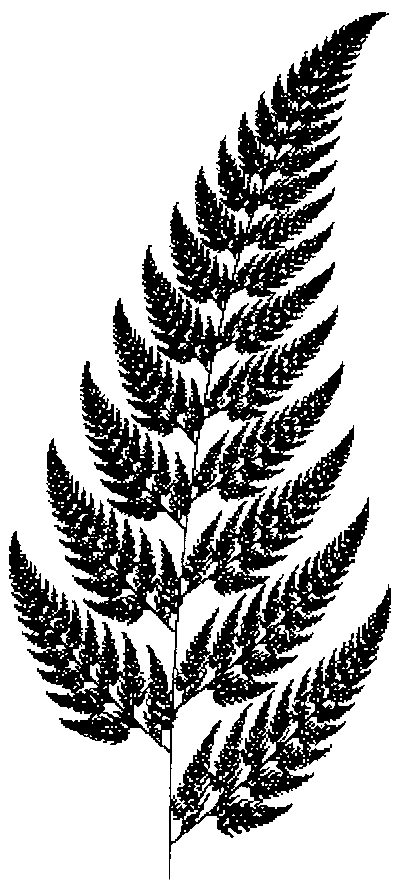
\includegraphics{Images/10-Fern}\label{Fern}}}
	\hspace{2cm}
	\subfloat[Julia Sets]{{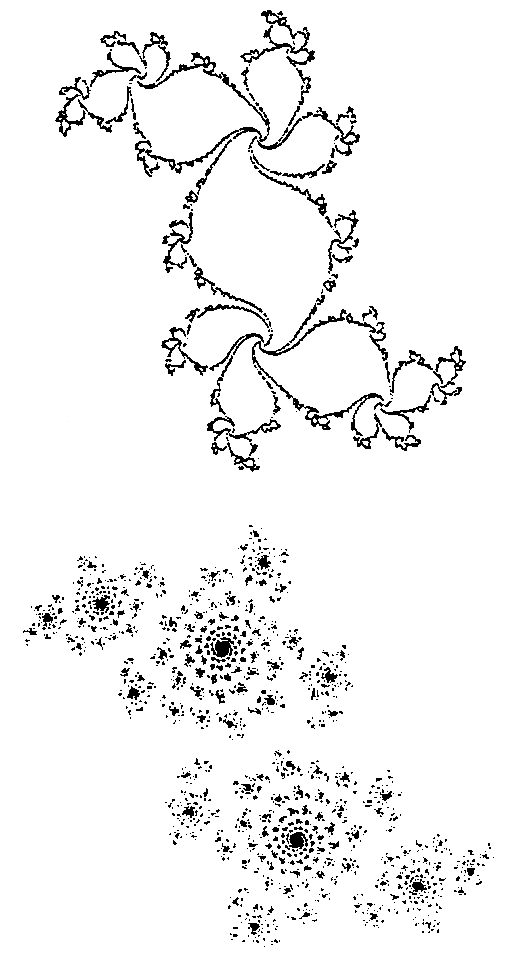
\includegraphics{Images/11-JuliaSets}\label{JuliaSets}}}
	\caption[Fractal Forms]{Fractal Forms \cite{falconer03}}
	\label{Fractal}
\end{figure}

\begin{figure}[htbp]
\centering
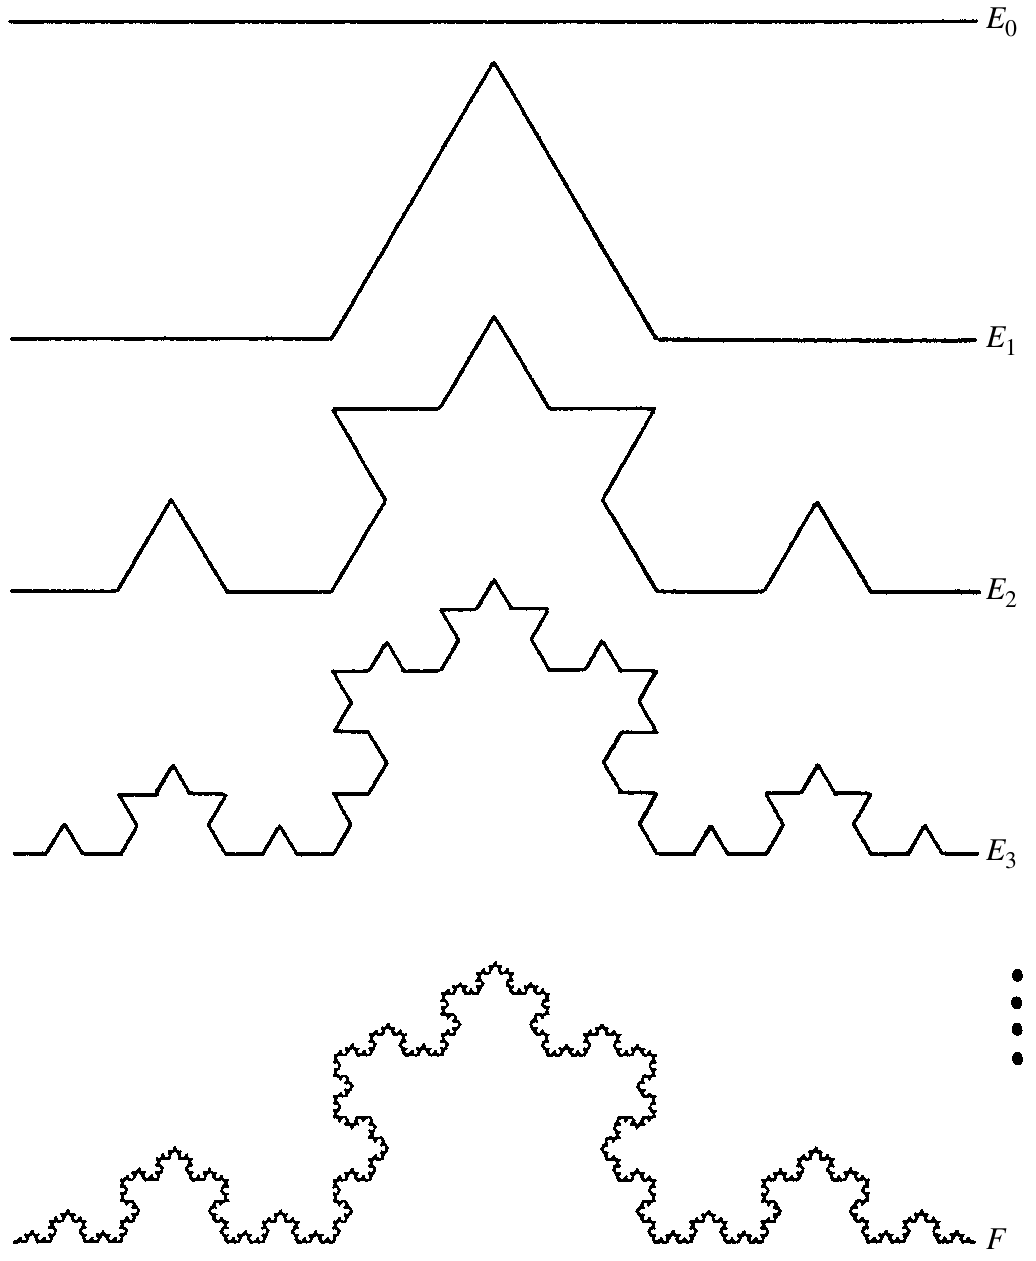
\includegraphics[width=0.8\textwidth]{./Images/9-FractalGeom}
\caption[The Koch Curve]{An example of fractal geometry: The Koch Curve \cite{falconer03}}
\label{KochCurve}
\end{figure}

Fractals are a naturally occurring phenomenon, such formations of snow flakes, clouds, fern leaves (Fig \ref{Fractal}\subref{Fern}) and coastlines. As mentioned before ; the derivation of generative systems from natural formations can be beneficial in optimisational terms of building performance (\emph{see page} \pageref{NaturalOpt}).

\clearpage
\subsection{Shape Grammars}

A project by George Stiny and James Gips in 1977; shape grammars were intended to be a scientific approach to the language and composition of design. The main goal of shape grammars was to make the design process detached from individuals' minds and externalised to something that can be transmitted and modified. A distinctive feature of shape grammars is the visual method of form generation rather than the symbolic or numerical.

As with cellular automata and fractals; the process of generation with shape grammars starts with an initial shape, and is transformed through a given rule. Rules in shape grammars take the form of: \begin{equation} A \rightarrow B \end{equation}
Whenever a shape matching the left side of the rule $A$ occurs, the rule is applied (Fig. \ref{ShapeGrammarsRule}). As described in a previous section, the type of transformation applied to the shape can addition, subtraction, rotation\ldots etc. 

\begin{figure}[htbp]
\centering
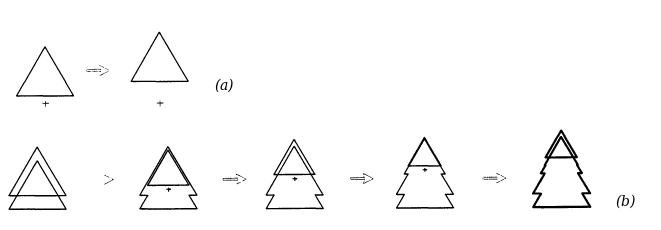
\includegraphics[width=\textwidth]{./Images/12-ShapeGrammarsRule}
\caption[Shape Grammars Rule]{A Shape Grammars Rule: \emph{(a) rule, (b) transformation} \cite{arida04}}
\label{ShapeGrammarsRule}
\end{figure}

Shape grammars also have the ability to apply the rules to emergent shapes; not predefined in the grammar. Shape grammars can be used as a synthesizer of shapes be generation, or as an analysis tool of complex shapes; decomposing them into simple ones. Among the many real world applications of shape grammars, a relatively new one was described by D. Shelden \cite{shelden02}; which was during the preparation of contract documents of the \emph{Experience Music} project. The case was the subdivision of a cladded surface for fabrication of the cladding sheets. The surface was divided using a shape grammar rule, but upon receiving the requirements of the fabricator which were smaller sheets; a different rule was used to subdivide the surface (Fig. \ref{SubdivisionSG} -- \ref{SubdFab}).

\begin{figure}[htbp]
\centering
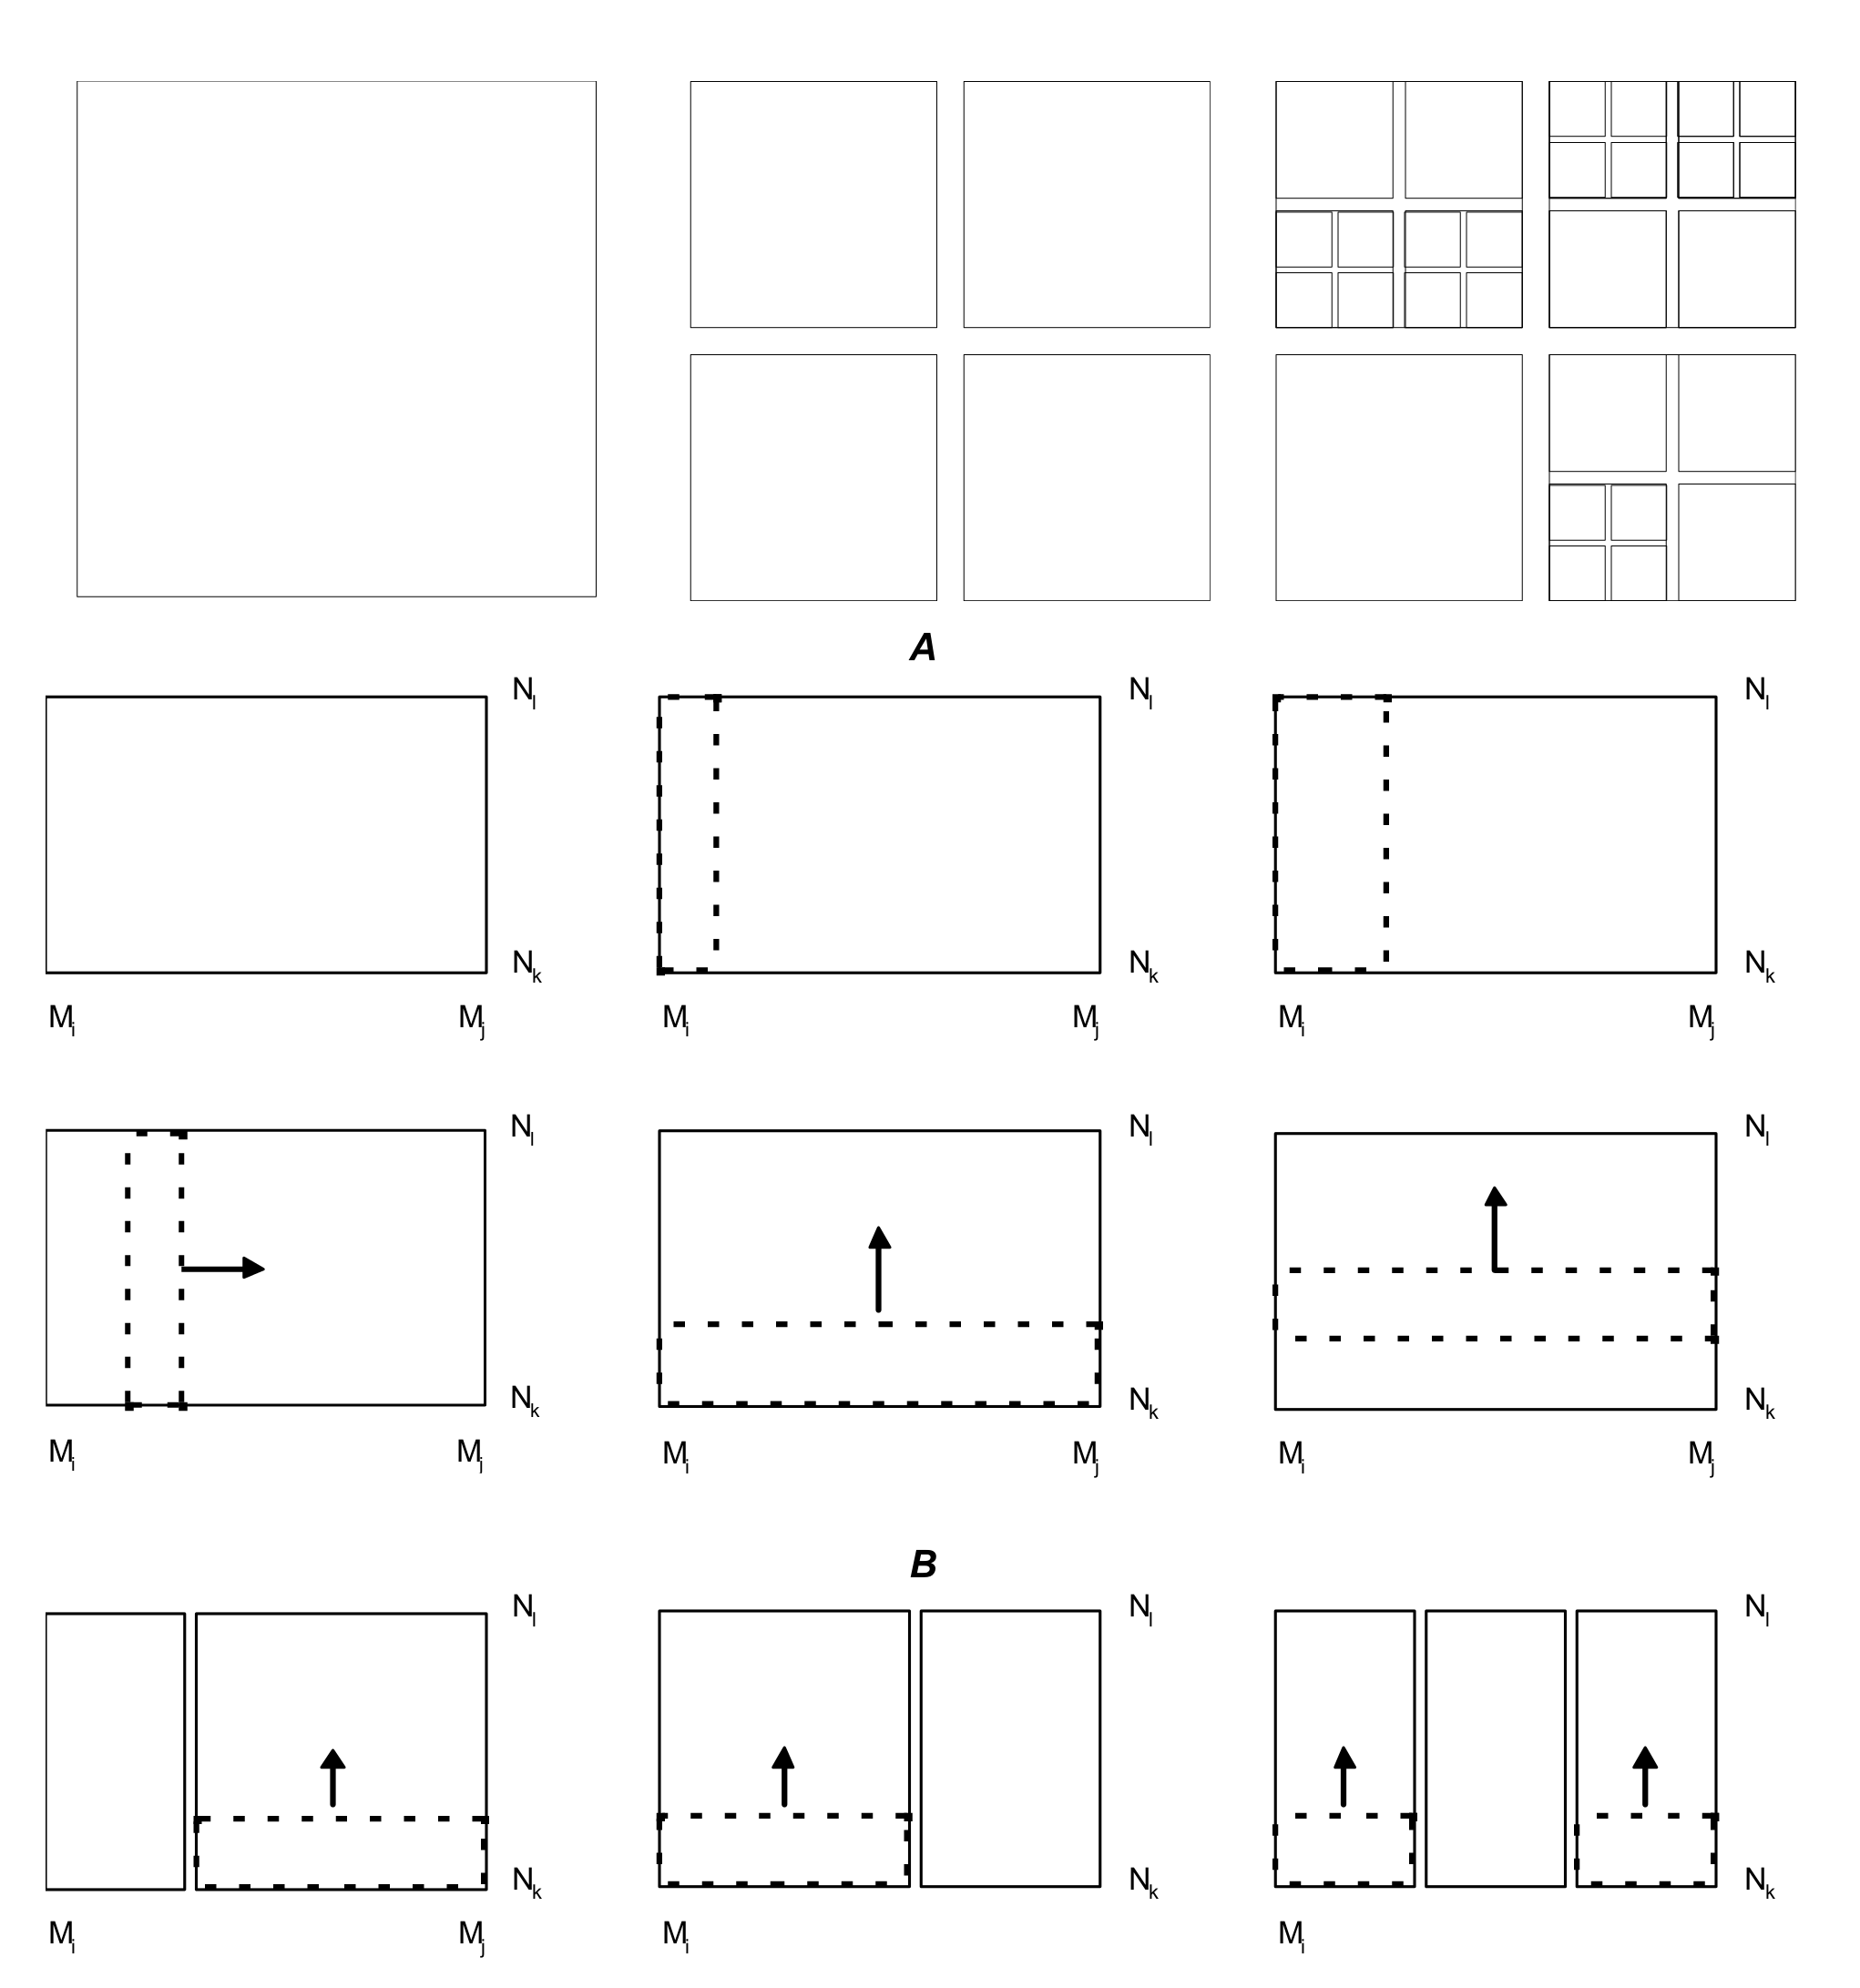
\includegraphics[width=0.5\textwidth]{./Images/13-SubdivisionRule}
\caption[Shape Grammar Subdivision]{The subdivision of a surface by shape grammars for fabrication of the sheets \cite{shelden02}}
\label{SubdivisionSG}
\end{figure}

\begin{figure}[htbp]
\centering
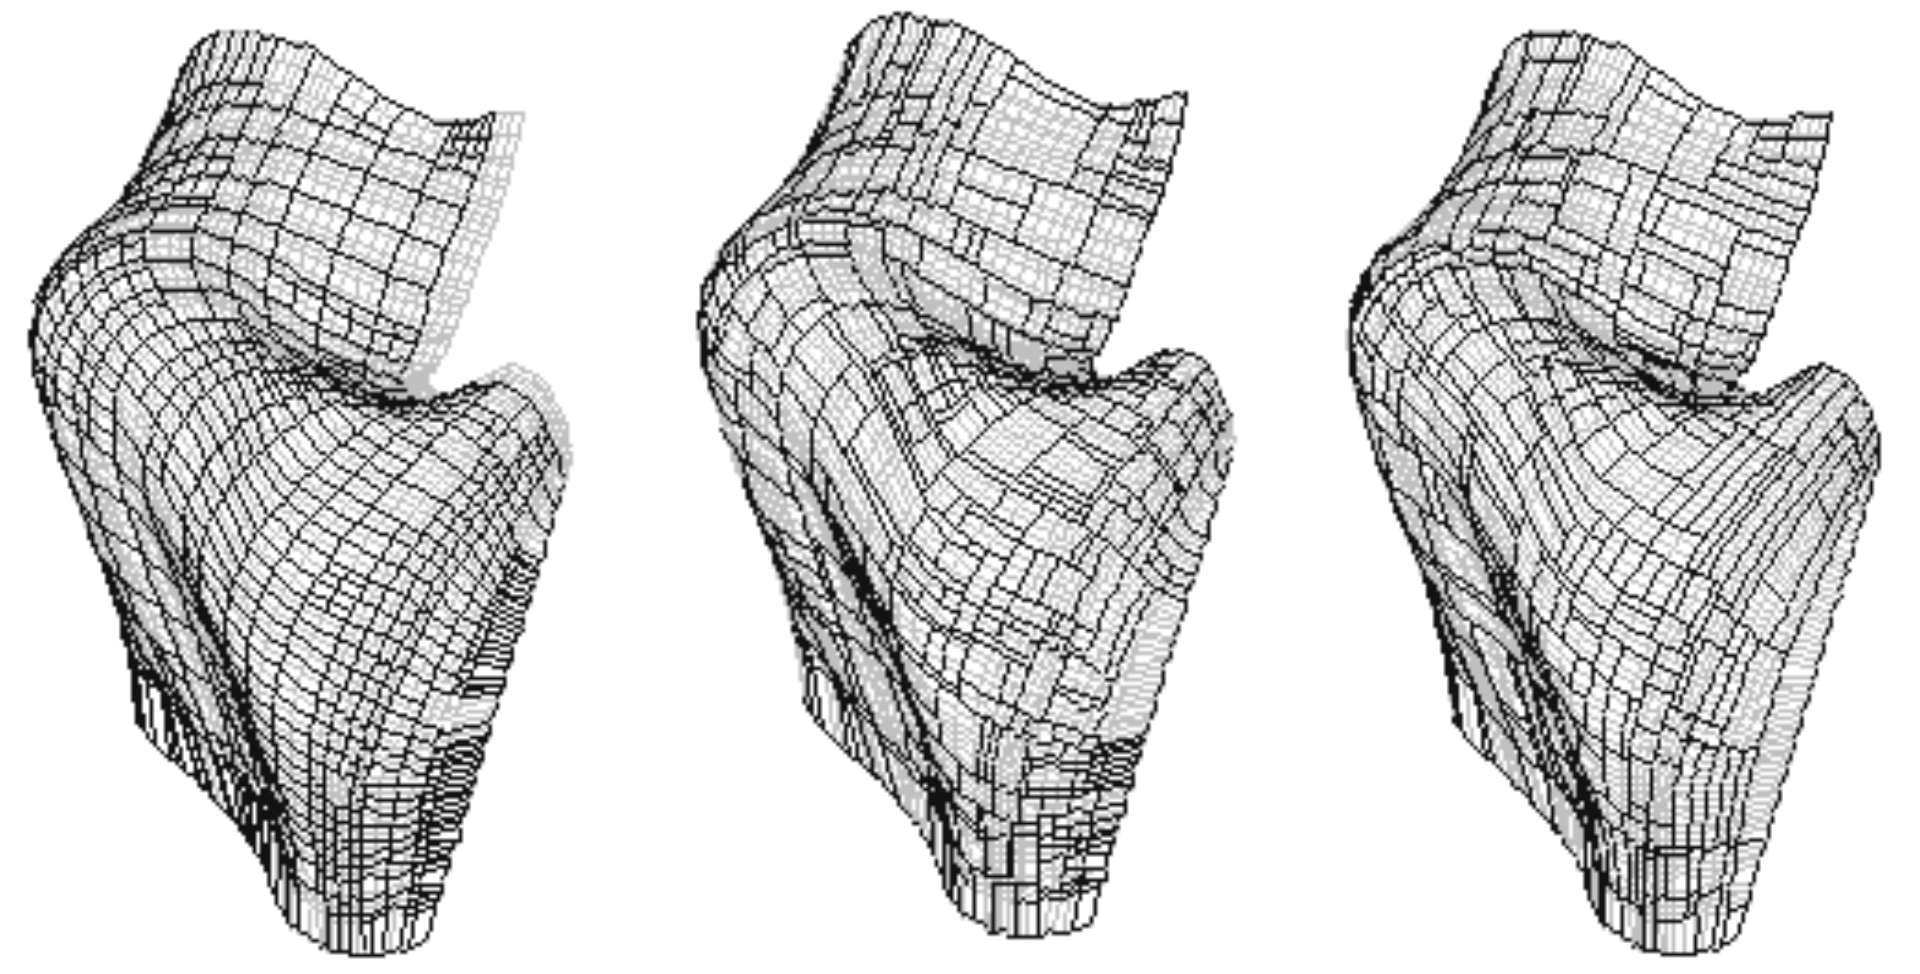
\includegraphics[width=\textwidth]{./Images/14-SurfaceFabrication}
\caption[Fabrication Surface Subdivision]{The subdivision of building envelope for fabrication \cite{shelden02}}
\label{SubdFab}
\end{figure}

\clearpage
\subsection{L-Systems}

L-System; an abbreviation of Lindenmayer-systems after Aristid Lindenmayer, was created in 1968 as a mathematical simulation of plant growth \cite{fasoulaki08}, consisting of four elements: \begin{inparaenum} \item a starting configuration string, \item a set of rules, \item constraints and \item variables.\end{inparaenum}

L-Systems are very similar to Shape Grammars, with the exception of being represented textually not spatially \cite{arida04}, but operate in a recursive manner such as that of Shape Grammars. The form by which rules of context-sensitive L-Systems is expressed is: \begin{equation} B<A>C\rightarrow X \end{equation}\ldots where $A$ would produce $X$ if and only if $A$ is surrounded by $B$ on the left and $C$ on the right. The rule form of context-independent L-Systems is: \begin{equation} A \rightarrow B \end{equation}

\begin{figure}[h]
\centering
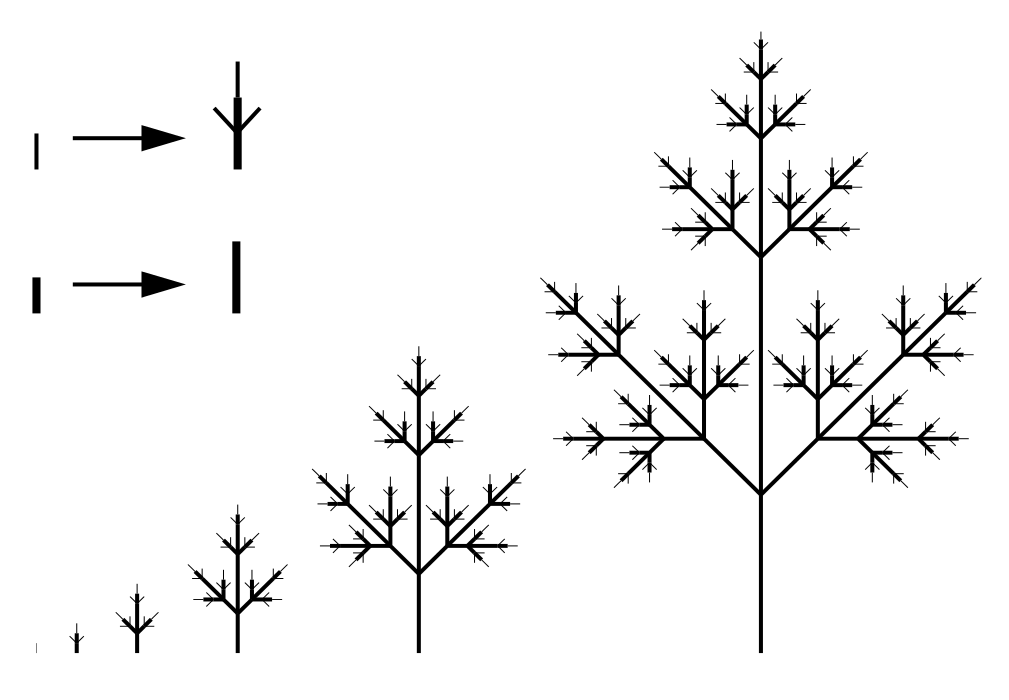
\includegraphics[width=\textwidth]{./Images/15-L-SystemLeaf}
\caption[L-System Compound Leaf]{Development of a compound leaf shape \cite{csiro96}}
\label{LSysLeaf}
\end{figure}

\subsection{Generative Algorithms Comparative Analysis}

Having discussed the different generative algorithms and other processes (including those in chapter 1), the following exerpted study \cite{khaldi04} (Table \ref{tab:GenerativeRecap}) forms a recapitulation as a comparaison in accordance with and under the taxonomy illustrated earlier in chapter 1 (Section \ref{GenSysTax}).

\begin{landscape}
\centering
\begin{longtable}{*{7}{p{0.121\linewidth}}}
 &\textbf{Algorithms}&\textbf{Prametric}&\textbf{L-Systems}&\textbf{Cellular Automata}&\textbf{Fractals}&\textbf{Shape Grammars}\\\midrule
\textbf{Context in Computing}&Varies&Regeneration&Botanic Growth&Reproduciton&Mathematical Monsters&Visual Calculation\\\midrule
\textbf{Computation}&Varies&Varies&Parallel&Sequential&Varies&Varies\\\midrule
\textbf{Design Components}&Generators/ Interpretors/ Evaluators&Generators/ Interpretors/ Evaluators&Generators/ Interpretors/ Evaluators&Generators/ Interpretors/ Evaluators&Initiators/ Constructors/ Evaluators&Initiators/ Constructors/ Evaluators\\\midrule
\textbf{System Behaviour}&Varies&Possible Inheritance&Deterministic or Non-Context-Sensitive or None&Periodic, Aperiodic, Chaotic, Random&Recurssive&Determisitc or None\\\midrule
\textbf{Rule Types}&Varies&Varies&Replacement&Replacement&Replacement&Replacement\\\midrule
\textbf{Unit Types}&Vaires&Varies&Symbols&Symbols&Symbols, Numbers&Shapes\\\midrule
\textbf{Smallest Units}&Varies&Varies&Alphabet&Cell&Zero or oints&Basic elements\\\midrule
\textbf{Means of Recognition}&Varies&Varies&Counting&Counting&Counting&Seeing\\\midrule
\textbf{Basic System Components}&Tasks and units&Algorithms and associations&Algorithms and replacement rules&Algorithms and replacement rules&Algorithms and replacement rules&Algorithms and replacement rules\\\midrule
\textbf{Inheritance}&Continous&Continous&Discrete&Discrete&Discrete&Continous\\\midrule
\textbf{Constraints}&Relationships&Relationships&Adjacent Letters&States, Neighbour, Location&Location, Stoping Conditions&Colours, Labels, Axis\\\midrule
\textbf{Solution Space}&Units, Tasks, Relationships&Parameters, Variables, Relationships&Rules, Generations, Replacing Alphabets&Rules, Time Steps, Cells, Neighbourhood Size&Rules, Stopping Conditions&Rules, Recognized Shapes, Replacing Shapes\\
\bottomrule
\caption[Analytical Comparison of Generative Systems]{Analytical Comparison of Generative Systems \cite{khaldi04}}
\label{tab:GenerativeRecap}
\end{longtable}
\end{landscape}

\clearpage
\section{Performative Algorithms}

Having observed some of the prominent methods of generative design, one could define performative design by saying that unlike generative methods, performative design deals with how the building performs; not how the building looks. Performative algorithms examines a specific aspect of any given building's performance and improves it. 

When speaking of green and sustainable design, performative design always comes to mind. However; it does not deal with the environmental impact of buildings, which rules out the capability of producing green design. Nevertheless; in recent years it has become the quintessential method of production of sustainable design. This owes to the fact that performative design, through simulation and selection can produce designs that are highly efficient at lowering energy consumption and waste production, in some cases to the point of reaching \emph{zero footprint}\footnote{Theoretical absolute self-sufficiency and zero impact (waste production, energy consumption\ldots etc.}.

Performative design differs from generative design in that it does not rely solely on an algorithm for generation, but uses optimisation and simulation as tools. These tools are the main subjects of discussion in this section.

\paragraph{Optimisation}is the selection of the \emph{optimum} solution. Optimisation is a widely used system in engineering, considered as a problem-solver; optimisational algorithms are called search methods. As mentioned in a previous section (\ref{ParallelLogic}), computers have the power to delve into what humans cannot; the power to solve problems with high complexity requiring enormous amounts of computation. These complex problems --- as far as this thesis is concerned --- will be mainly dealt with using \emph{Mathematical Optimisation}.

\newpage
\paragraph{Mathematical Optimisation} is the process of:
\vspace{-0.5cm}
\begin{enumerate}
\item the formulation and,
\item solution of a constrained optimisation problem of the general mathematical form:
\end{enumerate}
\vspace{-0.9cm}

\begin{equation}
\text{minimize }f(x),x=[x_1,x_2,\cdots,x_n]^T \in \mathbb{R}^n
\label{OptMathForm}
\end{equation}

\ldots subject to the constraints:
\begin{equation}
\begin{split}
g_j(x)\leq 0, j=1,2,\cdots,m \\
h_j(x)=0, j=1,2,\cdots,r
\label{OptConstr}
\end{split}
\end{equation}

\ldots where $f(x)$, $g_j(x)$ and $h_j(x)$ are scalar functions of the real \emph{column vector} \textbf{x}. \cite{snyman05}

``The continuous components of $x_i$ of \textbf{x} $=[x_1,x_2,\cdots,x_n]^T$ are called \emph{design} variables, $f(x)$ is the objective function, $g_j(x)$ denotes the respective \emph{inequality constraint functions} and $h_j(x)$ the \emph{equality constraint functions}.'' \cite{snyman05}

``The optimum vector \textbf{x} that solves the eqution (\ref{OptMathForm}) is donted by \textbf{x*} with corresponding optimum function value $f(\text{\textbf{x*}})$. If no constraints are specified, the problem is called an \emph{unconstrained} minimization problem.'' \cite{snyman05}

Mathematical optimisation is also called \emph{Nonlinear Programming, Mathematical Programming} or \emph{Numerical Optimisation}. As stated earilier; optimisation is a science that determines the best solutions, which in this case is to a mathematically defined problem that can be models of physical reality or otherwise. Mathematical optimisation tends to find the solution corresponding to minimum energy configurations of general structures, from molecules to suspension bridges, making it of great value to scientists and engineers.

The values of the functions $f(x)$, $g_j(x)$ and $h_j(x)$ (equations \ref{OptMathForm} and \ref{OptConstr}) may be obtained at any point $x$ using:
\vspace{-0.5cm}
\begin{enumerate}
\item analytical formulae (e.g. $f(x)=x_1 ^2+2x_2 ^2+\sin x_3$),
\item the outcome of a complicated computational problem (finite element analysis of stress) or
\item measurements taken from a physical process
\end{enumerate}
\vspace{-0.5cm}

These methods fall under different classes of solving the general problem, which might be analytically or numerically, while numerical methods being more common through different computational algorithms. The method of choosing the more suitable algorithm (also known as mathematical modelling) is depicted in figure (\ref{fig:MathModProc}).

\begin{figure}[htbp]
\centering
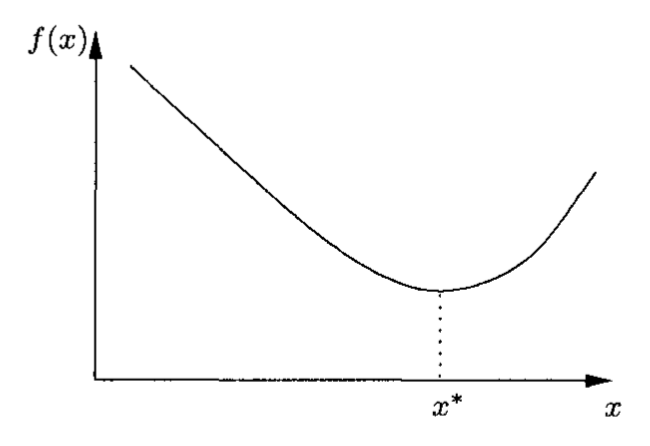
\includegraphics[width=0.7\textwidth]{./Images/19-FunctionOpt}
\caption[Function of Single Variable]{Function of single variable with optimum at $x^*$ \cite{snyman05}}
\label{fig:FunctionOpt}
\end{figure}

\begin{sidewaysfigure}[htpb]
\centering
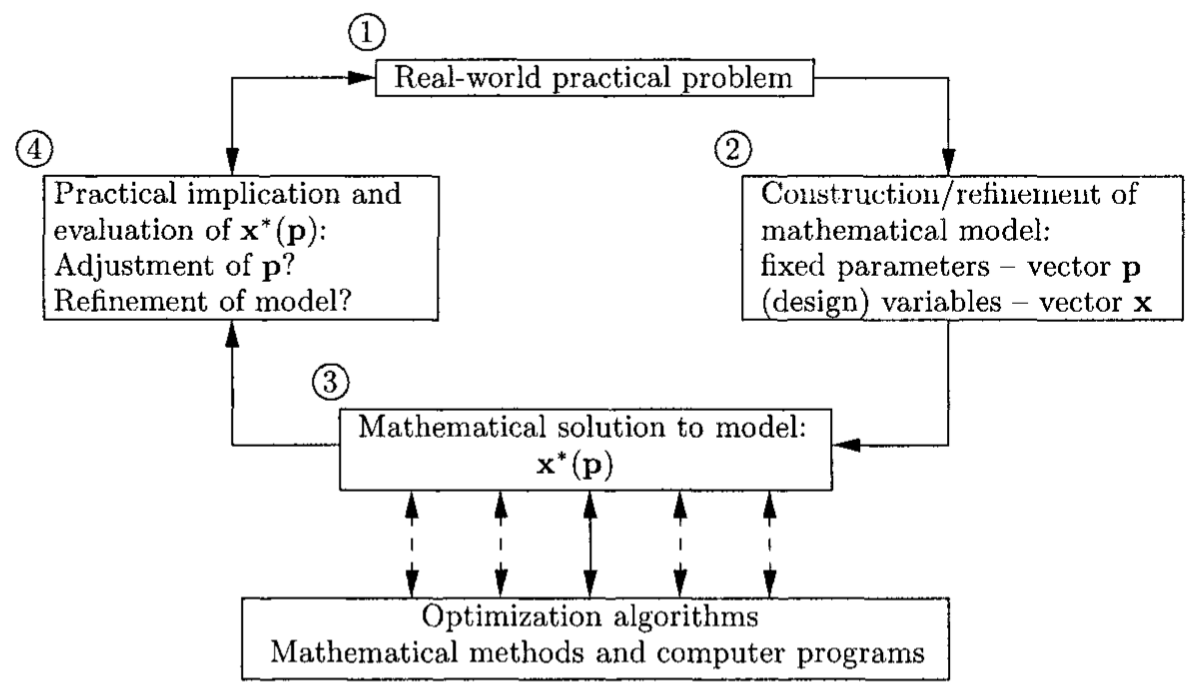
\includegraphics[width=\textheight]{./Images/18-MathModProc}
\caption[Mathematical Modelling]{The Mathematical Modelling Process (refer to fig. \ref{fig:FunctionOpt}) \cite{snyman05}}
\label{fig:MathModProc}
\end{sidewaysfigure}

The following section will discuss popular optimisation algorithms in architecural design, which are --- on an abstract level --- mathematical optimisation methods. Several subsets of optimisation exist, including \emph{Combinatoral, Linear, Nonlinear, Convex} and \emph{Metaheuristic}. The methods discussed herein will be of the \emph{Heuristic/Metaheuristic} subset.

\clearpage
\subsection{Genetic Algorithm}
\label{subsec:GA}

Genetic algorithm is an evolutianary algorithm, a subset of heuristic\footnote{Of or relating to exploratory problem-solving techniques that utilise self-educating techniques to improve performance\cite{merriam03}} search methods for solving optimisation problems, simulating biological evolution \cite{fasoulaki08}. Genetic Algorithm has unique terminology due to it's origins in biological evolutionary science.

``Under GA terminology, a solution to a problem is an \emph{individual}, and the group solutions existent at each stage is a \emph{population}. Each time a new population of individuals is created is called a \emph{generation}. In binary GAs\ldots each individual is represented by a binary string called a \emph{chromosome}, which encodes all parameters of interest corresponding to that individual. A chromosome is formed of \emph{alleles}; the binary coding bits. The fitness of any particular individual corresponds to the value of the objective function at that point''. \cite{caldas01}

\begin{figure}[htbp]
\centering
\begin{tikzpicture}[node distance=1.5cm, auto]
\node [rectangle, draw, rounded corners, minimum height=1cm] (init) {Generating Initial Population};
\node [rectangle, draw, rounded corners, minimum height=1cm, below of=init] (scaling) {Scaling};
\node [rectangle, draw, rounded corners, minimum height=1cm, below of=scaling] (select) {Selection};
\node [rectangle, draw, rounded corners, minimum height=1cm, below of=select] (cross) {Crossover};
\node [rectangle, draw, rounded corners, minimum height=1cm, below of=cross] (mutation) {Mutation};
\node [rectangle, draw, rounded corners, minimum height=1cm, below of=mutation] (elit) {Elitist Model};
\node [shape=diamond, draw, shape aspect=2, node distance=2.5cm, below of=elit] (term) {Termination Condition};
\node [shape=circle, draw, shape aspect=2, node distance=2.5cm, below of=term] (end) {End};

\draw [-latex', thick] (init) -- (scaling);
\draw [-latex', thick] (scaling) -- (select);
\draw [-latex', thick] (select) -- (cross);
\draw [-latex', thick] (cross) -- (mutation);
\draw [-latex', thick] (mutation) -- (elit);
\draw [-latex', thick] (elit) -- (term);
\draw [thick] (term) -- (-4,-10);
\draw [thick] (-4,-10) -- (-4,-1.5);
\draw [-latex', thick] (-4,-1.5) -- (scaling);
\draw [-latex', thick] (term) -- (end);
\node [above] at (-3.5,-10) {No};
\node [left] at (0,-11.6) {Yes};
\end{tikzpicture}
\caption[Genetic Algorithm Flowchart]{The sequence and loop of GA's}
\label{GAFlw}
\end{figure}

The process of problem solving in GA is fairly simple (Fig \ref{GAFlw}), despite it's ability to solve highly complex problems. Initially; a population is randomly generated with a sufficient amount of chromosomes allowing for a wealth of genetic information to be processed and therefore statistically provides a better solution, although the bigger the population; the more computing power is needed. 

Individuals are then selected on a basis of fitness defined by the user prior to the process. At this stage, a number of genetic operators (stochastic operators) become in effect, such as \emph{crossovers} (fig. \ref{CRSOVR}). Crossovers are swapping of parts of two chromosomes selected for their fitness, producing a new offspring of individuals containing some genetic material from each \emph{parent} individual. This process is repeated and reiterated to produce more refined generations gradually through selection.

Another function of GA is \emph{mutation}, which occurs randomly at a predefined to affect some chromosomes in the intermediate phase between any two crossovers. The idea of mutation is to introduce alterations to the selection of chromosomes, and therefore allowing for genetic diversity at later stages of the selection process, assisting the search by escaping the local optima. Nevertheless, it's frequency is adjusted as to allow for genetic diversity without producing a generation of crossovers that is completely different from it's predecessor.

At the final stage of the search process, an elitist model is created and presented as the `best' set of solutions, which meet the termination criteria; ending the search. The difference between GA and traditional  search methods, is that GA is a probabilistic search method, not a deterministic one, which searches through a population in different points in parallel not a single point. However, genetic algorithm is very robust due to the fact that it needs little information about the design problem, and is efficient when the population space is large and complex, which no traditional mathematical search method can process. This is however at the cost of knowing that the given solution is the best within the population, but not the optimum solution.

\paragraph{Crossover.} The following table illustrates the swapping technique of crossover between two individual chromosomes.

\begin{table}[h]
\begin{tabular}{l|| ccccc|ccccccccccc}
\textbf{Parent 1}&1&1&0&1&0&0&1&1&0&0&1&0&1&1&0&1\\
\textbf{Parent 2}&y&x&x&y&y&x&y&x&x&y&y&y&x&y&x&x\\\hline
\textbf{Offspring 1}&y&x&x&y&y&0&1&1&0&0&1&0&1&1&0&1\\
\textbf{Offspring 2}&1&1&0&1&0&x&y&x&x&y&y&y&x&y&x&x\\
\end{tabular}
\caption[Crossover Operative]{Crossover Operative \cite{whitley94}}
\label{CRSOVR}
\end{table}

The range of application of GA in architecture are wide, with a prominent success in the fields of energy consumption and structural analysis. A common practice in problem solving with GA is coupling it with a problem dependant simulation (to be discussed further in this chapter), providing feedback to refine the initial population.

An example of GA implementation in passive solar design is the model presented by Go Kawakita \cite{kawakita08}. The optimisational problem addressed the fenestration of a building envelope under a specific set of environmental conditions (fig \ref{kawakitaGA}). The variables --- or parameters --- studied in the process were the size, shape, shape iteration and location of openings, which was evaluated prior to and after GA optimisation using ECOTECT simulation, which feedback the results for re-optimisation in case of the optimised model not meeting the process termination criteria.

\clearpage
\subsection{Simulated Annealing}

Simulated annealing is a mathematical optimastion method. It draws it's terminology from the metallurgical process of annealing which is the heating and controlled cooling of metals to reach it's ground state with the lowest internal energy without being trapped in the local minimum \cite{lam88}. It was originally introduced by S. Kirkpatrick in 1982. The method is metaheuristic\footnote{A method that guides another heuristic (self learning) optimisational method}, used for maximisational and minimisational optimisation problems, which tend to find the global optimum (minimum or maximum).

Local and global minima and maxima are mathematical terms describing the highest (maxima) and lowest (minima) values of a given function, within either a defined range (local) or the entire function domain. The idea behind simulated annealing --- as with the physical process --- is to find the global rather than the local minimum; i.e. to find a better state than the initial one, through a technique called \emph{descent method} (the heuristic method which SA drives as mentioned)  which incrementally replaces the initial state with a set of predefined ones.

As with genetic algorithm, the original source of inspiration heavily influences the terminology and the process of simulated annealing, which mimics metal annealing to the extent of the algorithm pseudocode (Algorithm \ref{SimAnn}) being an identical description of the physical process.

\begin{algorithm}
\begin{algorithmic}[1]
\State Get an initial state with energy $x$
\State Make the initial state the current state
\State Select an initial high temperature $T$
\While {System is not yet frozen}
	\While {System is not yet in thermal equilibrium}
		\State Pick a random nearby state with energy $x_p$
		\State Let $\Delta x = x_p - x$
		\If {$\Delta x \leq 0$}
			\State The new state becomes the current state
		\Else
			\State Reject state
		\EndIf
	\EndWhile
	\State Reduce temperature $T$ by $\Delta T$
\EndWhile
\State Output the current state
\end{algorithmic}
\caption{Simulated Annealing Method \cite{lam88}}
\label{SimAnn}
\end{algorithm}

\clearpage
\subsection{Tabu Search}

While Genetic Algorithms (GAs) imitate the phenomenon of biological reproduction, and Simulated Annealing (SA) is based on physical process in metallurgy; the philosophy of Tabu search (TS) is to derive and exploit a collection of principles of intellegant problem solving; it is based on selected concepts that unite the fields of artificial intellegance and optimisation. \cite{glover97}

``Tabu search is a meta-heuristic that guides a local heuristic search procedure to explore the solution space beyond the local optimality. \ldots The local procedure is a search that uses an operation called \emph{move} to define the neighbourhood of any given solution. One of the main components of TS is its use adaptive memory, which creates a more flexible search behaviour. Memory-based strategies are therefore the hallmark of tabu search approaches.'' \cite{glover97}

``Tabu search is based on the premise that problem solving, in order to qualify as intelligent, must incorporate \emph{adaptive memory} and \emph{responsive exploration}. A good analogy is moutain climbing, where the climber must selectively remember key elements of the path traveled (using adaptive memory) and must be able to make strategic choices along the way (using responsive exploration). The adaptive memory features of TS allows the implementation of procedures that are capable of searching the solution space economically and effictively. Since local choices are guided by information collected during the search, TS contrasts with memoryless designs that heavily rely on semi-random processes that implement a form of sampling. Examples of memoryless include \ldots traditional annealing and evolutionary approaches.'' \cite{glover97}

\paragraph{Use of Memory.} The memory structures in tabu search operate by reference to four main elements: \emph{recency, frequency, quality} and \emph{influence}.

\begin{enumerate}
\item \emph{Recency-based} memory is a type of short memory that keeps track of the attributes of recently visited solutions. These attributes are then labeled \emph{tabu-active}. This prevents visited solutions or the paths leading to them to be revisited.
\item \emph{Frequency-based} memory provides a type of information that complements the information provided by recency-based memory, broadening the foundation for selected preferred moves.
\item The \emph{quality} dimension refers to differentiate the merit of solutions vistied during search. Memory can then be used to identify elements that are common to good solutions or to paths that lead to them. This in turn reinforces the search to obtain the best results within the solution space.  
\item \emph{Influence} considers the impact of the choices made during the search, not only on quality, but also on structure. Recording information about the influence of choices on particular solution elements incorporates and additional level of learning.
\end{enumerate}

The memory used in tabu search is both \emph{explicit} and \emph{attributive}. Explicit memory records complete solutions, typically consisting of elite solutions visited during the search. An extension of this memory records highly attractive but unexplored neighbours of elite solutions. Attributive memory on the other hand, is used for guiding purposes. This type of memory records information about solution attributes that change in moving from one solution to another.

\paragraph{Intensification and Diversification.} Intensification is linked with short term memory and explicit memory; it evaluates recently visited solutions and chooses to intensify search in a particular zone of the solution space when it detects that a large number of elite solutions, this zone could be called a neighbourhood, but with a different definition than usual; this neighbourhood consists of all solutions within this area regardless of their attributes. Diversification --- on the other hand --- encourages the search process to investigate unvisited regions, and generate solutions that are significantly different from previous solutions.

\clearpage
\subsection{Optimisation Search Method Comparison}
\label{subsec:OptimComp}

The following study (Table \ref{tab:OptCmp}) by L. Caldas \cite{caldas01} illustrates the characteristics of Genetic Algorithm, Simulated Annealing and Tabu Search; comparing them in terms of memory usage, intensification, diversification and neighbourhoods:

\begin{landscape}
\centering
\begin{longtable}[h]{p{1cm}*{4}{p{4.5cm}}}
\toprule\\ 
 &\textbf{Memory}&\textbf{Intensification}&\textbf{Diversification}&\textbf{Neigbourhood}\\ \midrule
\textbf{GA}&Some use of memory&Non-systematic&Crossover: New points in the solution space are created by combining existing solutions&No definition of neighbourhood\\
 &Explicit --- Elitism&Mutations: Introduces a small change to an existing solution, meaning it is searching in its vicinity&MicroGA's have high diversification by often starting new random populations&New solutions are found by the process of crossover between two existing solutions\\
 &Implicit --- Keeps track of high performance building blocks; sequence of generations propagates useful genetic information& & & \\\midrule
\textbf{SA}&Almost no use of memory&Search moves less freely as it progresses, with lower probability of accepting very different solutions from the current one&At early stages of the search, probability of accepting solutions that significantly decrease performance is higher, meaning that new regions of the search space are explored.&Requires a definition of a neighbourhood\\
 &Only if the best soution found so far is used to restart search after each temperature reduction&Neighbourhood radius can also decrease& &Size of neighbourhood is not too important, as not all of the neighbourhood is explored (at each step, a single solution is picked for evaluation)\\\midrule
\textbf{TS}&Extensive use of memory&Systematic&Systematic&Requires a definition of neighbourhoods\\
 &Recency-based: keeps track of recent moves to prevent reverse ones&Stores good configurations and then explores their neighbourhoods more thoroughly&Temporary change of rules can penalise solutions similar to the current one&Neighbourhood size is more critical, since it is a greedy algorithm that explores all of a single neighbourhood for best path\\
 &Frequency-based: keeps track of frequency of certian features in solutions already visited. Used for diversification&Path relinking: building blocks from elite solutions stored in memory can by used to produce new attractive solutions&Can be implemented by removing some features of the current solution that temporarily become tabu-active, thus forcing the search to visit previously unexplored regions&May include some method to explore only more attractive areas of the neighbourhood, like first randomly sampling neighbourhood and then exploring only the best solution areas\\
 &Quality memory: stores which building blocks to high quality solutions. Used for path relinking& & & \\
 &Influence memory: records impact of certain moves and makes bad moves tabu-active for some period of time& & & \\
\bottomrule
\caption[Optimisation Search Method Characteristics]{A comparison of optimisation search methods \cite{caldas01}}
\label{tab:OptCmp}
\end{longtable}
\end{landscape}

\clearpage
\subsection{Additional Search Methods}

In the previous sections three heuristic optimisation search methods have been discussed. However, it should be noted that other search methods that belong or do not belong to the heuristic/metaheuristic subset of search methods exist, which have not been discussed herein.

Other heuristic search methods indlude: \emph{Ant colony algorithms, Bee algorithms, Particle Swarm optimisation, Harmony search} and \emph{Firefly algorithm}.

In addition, other optimisation methods which do not fall under the category of heuristic methods include: \emph{Convex optimisation, Monte Carlo methods, Random Walk / Markov Chain}\ldots among others.

Although the three discussed were deemed sufficient for illustrative purposes within this thesis, it would be highly beneficial to examine the abovementioned search methods, as different methods will vary in compatability or suitability to different problems.

The next chapter will discuss the second foremost subject of this thesis; which is thermal design, from a physical, physiological, design process and variable points of view, which will integrate the full backround of this thesis's subject. 

The following chapter will introduce the different application methods of the discussed algorithms in the field of architectural design, and case studies of these applications.
